% !TeX spellcheck = en_US
\documentclass[french]{yLectureNote}

\title{Électrocinétique}
\subtitle{Physique}
\author{Paulhenry Saux}
\date{\today}
\yLanguage{Français}

\professor{Allard}%allard@irsamc.ups-tlse.fr
\usepackage{graphicx}%----pour mettre des images
\usepackage[utf8]{inputenc}%---encodage
\usepackage{geometry}%---pour modifier les tailles et mettre a4paper
%\usepackage{awesomebox}%---pour les boites d'exercices, de pbq et de croquis ---d\'esactiv\'e pour les TP de PC
\usepackage{tikz}%---pour deiffner + d\'ependance de chemfig
\usepackage{tkz-tab}
\usepackage{chemfig}%---pour deiffner formules chimiques
\usepackage{chemformula}%---pour les formules chimiques en \'equation : \ch{...}
\usepackage{tabularx}%---pour dimensionner automatiquement les tableaux avec variable X
\usepackage{awesomebox}%---Pour les boites info, danger et autres
\usepackage{menukeys}%---Pour deiffner les touches de Calculatrice
\usepackage{fancyhdr}%---pour les en-t\^ete personnalis\'ees
\usepackage{blindtext}%---pour les liens
\usepackage{hyperref}%---pour les liens (\`a mettre en dernier)
\usepackage{caption}%---pour la francisation de la l\'egende table vers Tableau
\usepackage{pifont}
\usepackage{array}%---pour les tableaux
\usepackage{lipsum}
\usepackage{yFlatTable}
\usepackage{multicol}
\newcommand{\Lim}[1]{\lim\limits_{\substack{#1}}\:}
\renewcommand{\vec}{\overrightarrow}
\begin{document}

	\chapter{Théorèmes de base}
\section{Appliquer le principe de superposition}
On cherche la tension dans un circuit
\begin{itemize}
 \item On compte le nombre de générateur (de tension ou de courant)
 \item On passive tous les générateurs de courant en les remplaçant par des intérrupteurs ouverts et les générateurs de tension par des intérrupteurs fermés, sauf un.
 \item Souvent, on peut alors simplifier le circuit en introduisant des résistances équivalentes puis en utilisant un pont diviseur de tension/courant.
 \item Dans chaque cas, on calcule la valeur qui nous interesse.
 \item On somme toutes les valeurs trouvées pour trouver la valeur finale.
\end{itemize}
Prenon cet exemple :

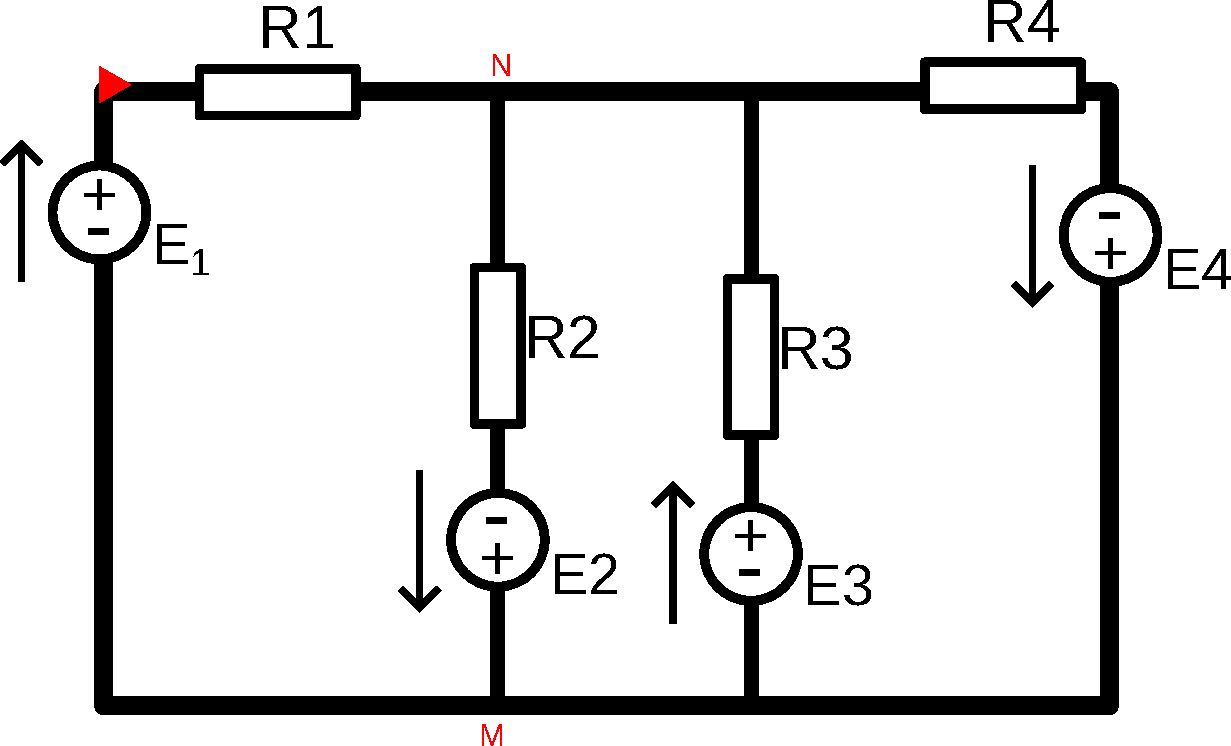
\includegraphics[scale=0.3]{methode-2-1}

Dans cet exemple, on cherche la tension NM. Pour cela, on va passiver tous les générateurs sauf \(E_1\) et calculer la tension.

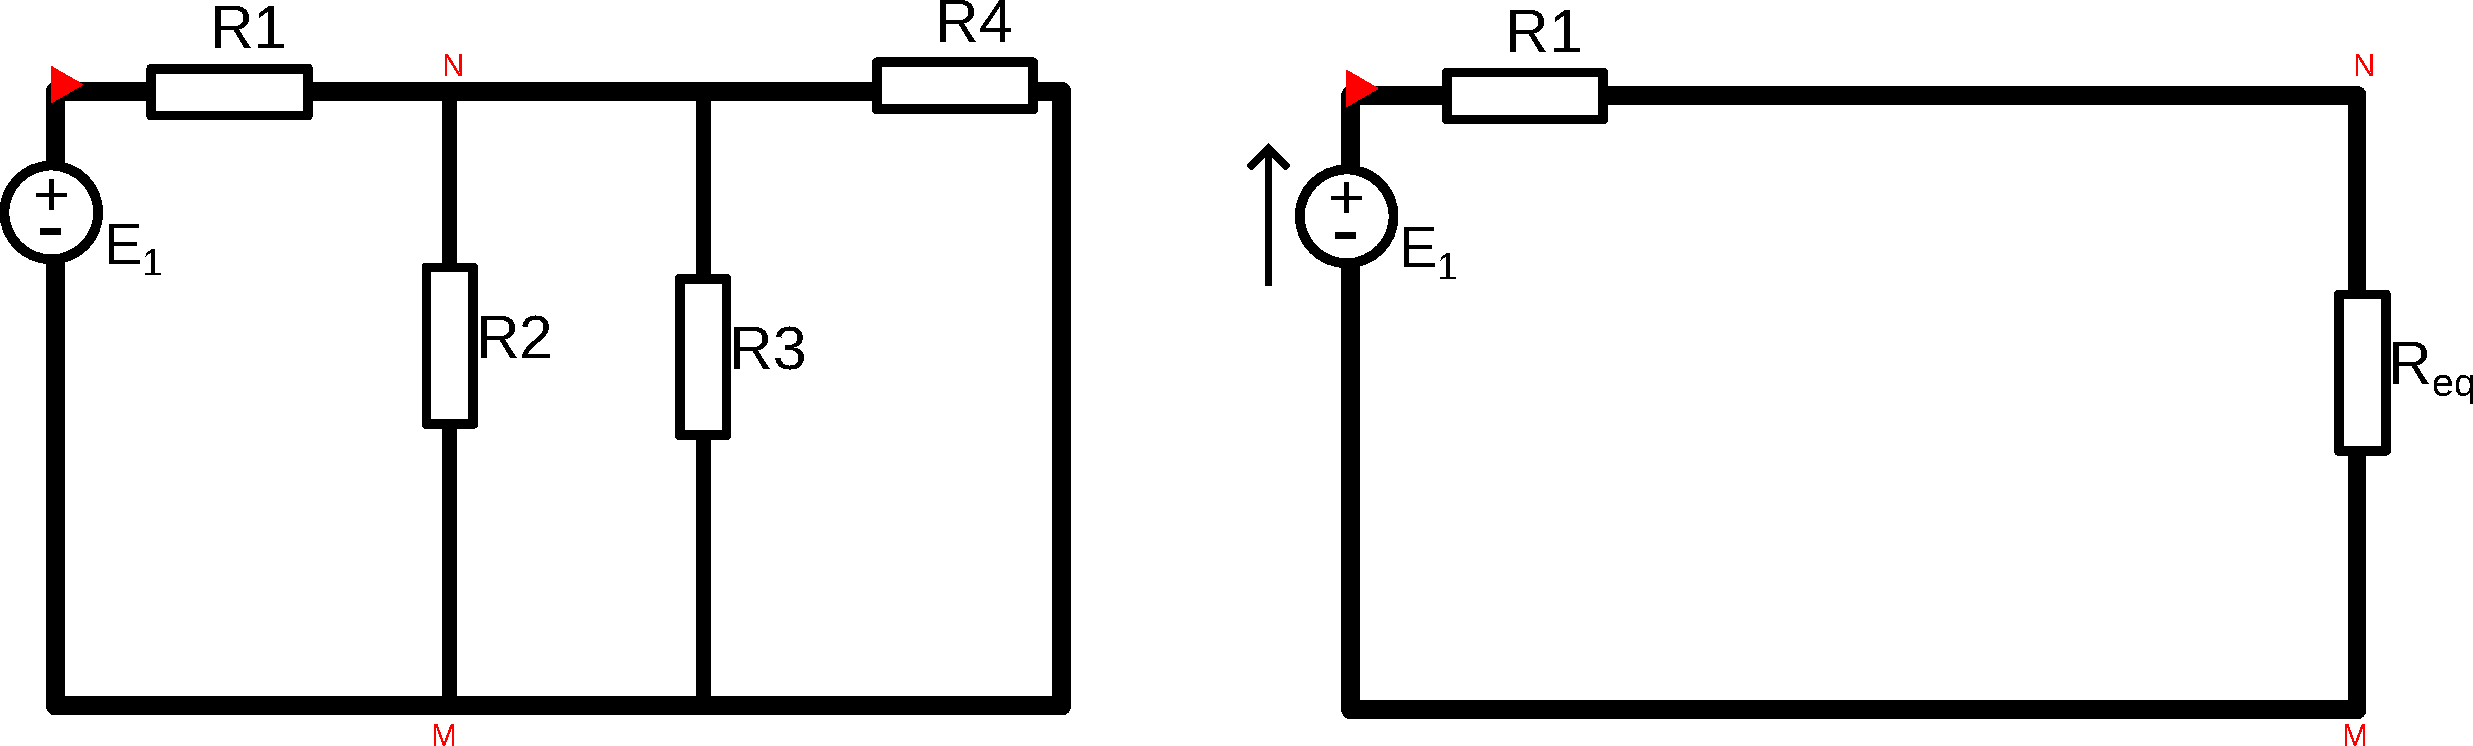
\includegraphics[scale=0.3]{methode-2-2}

Le circuit se simplifie et on peut calculer la résistance équivalente \(R_{eq} = \frac{1}{G_2+G_3+G_4}\). On applique ensuite un pont diviseur de tension pour trouver que \(U_{NM} = E_1 \times \frac{R_{eq}}{R_1+R_{eq}}\). On a donc obtenu la tension si seul le générateur 1 était fonctionnel. Il ne nous reste plus qu'à faire de m\^eme pour les 3 autres générateurs et sommer les quatre résultats.

\section{Appliquer le théorème de Thévenin et Norton}
\warningInfo{Remarque}{On n'appliquera ici que le théorème de Thévenin, mais il est possible de passer au cricuit de Norton avec les relations d'équivalence}
\begin{itemize}
 \item Pour trouver la résistance équivalente, on passive tous les générateurs, et on la cherche en faisant le parcours de A jusqu'à B.
 \item Pour trouver la tension équivalente, on débranche ce qu'il y a entre A et B, et on cherche la tension entre ces deux points
\end{itemize}
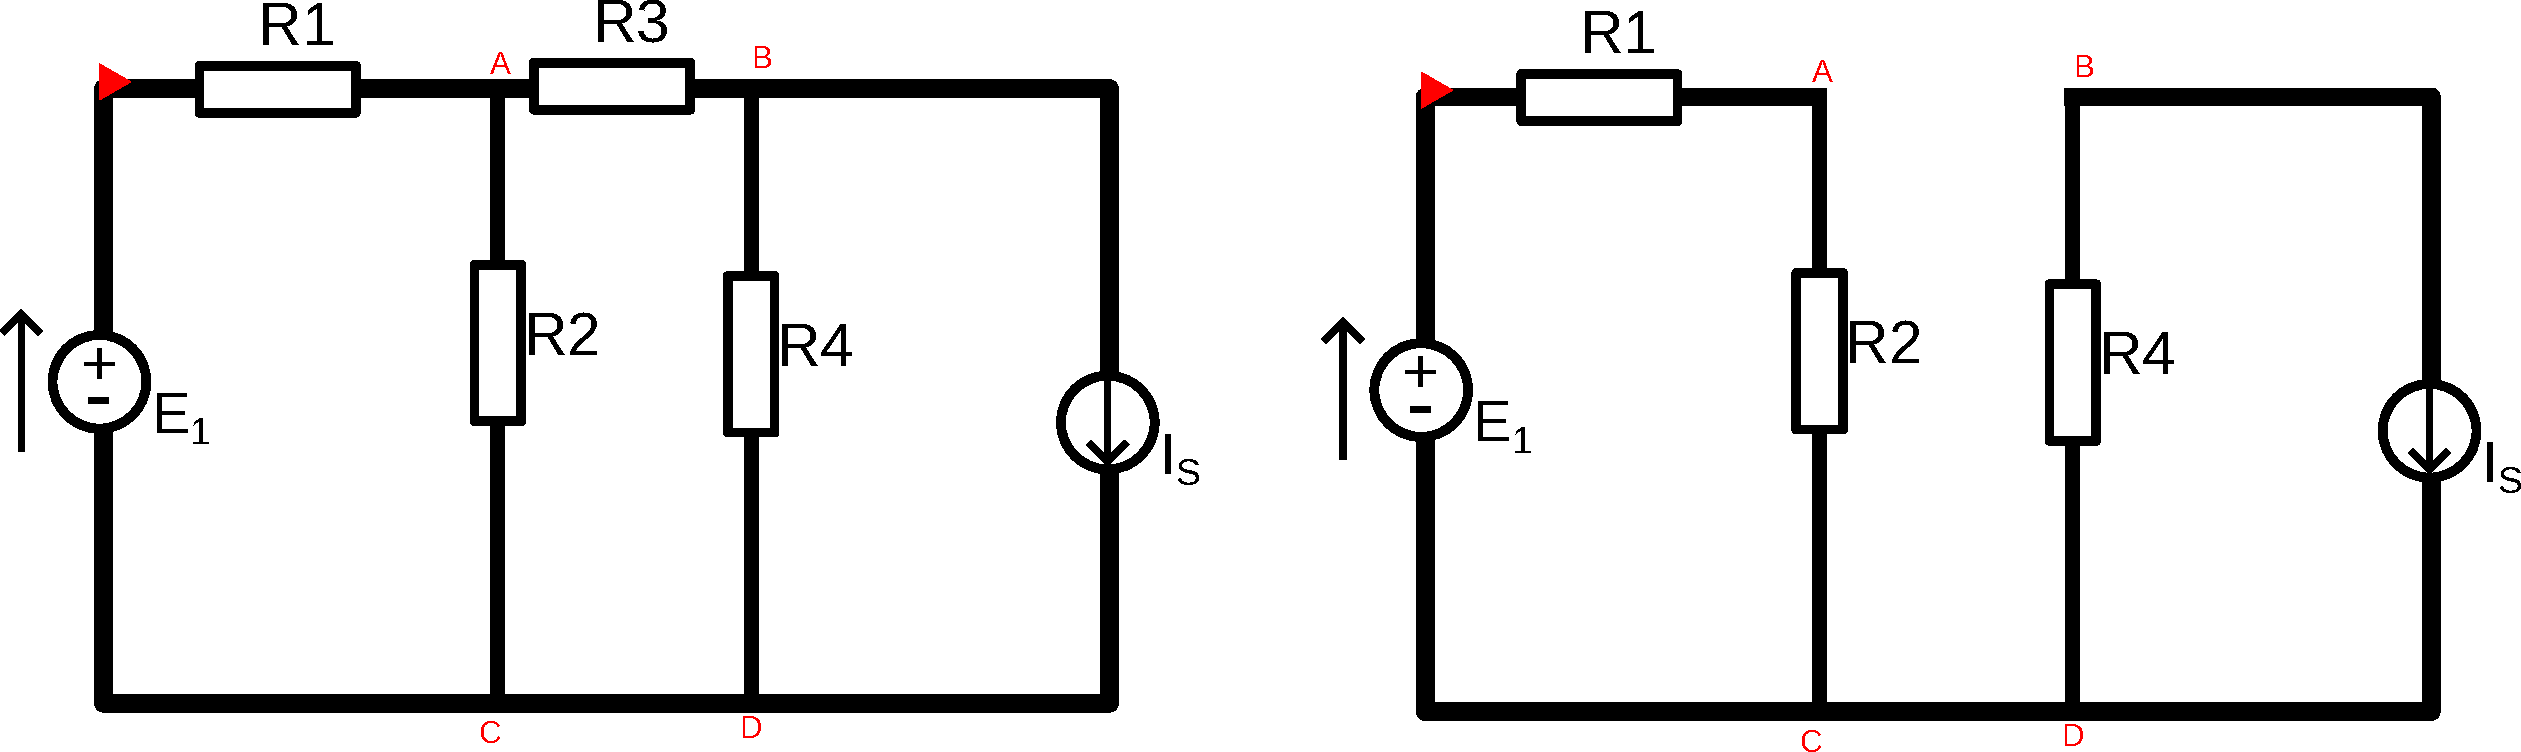
\includegraphics[scale=0.3]{methode-2-3}

Dans cet exemple, le but est de déterminer le courant traversant la résistance \(R_3\). On pourrait le faire en appliquant les lois des noeuds et des mailles, mais on va plut\^ot utiliser le théorème de Thévenin. On enlève donc la branche contenant la résistance \(R_3\) du circuit. On remarque tout de suite que le courant traversant la branche CD est nul, car la partie droite du circuit n'est connectée qu'une fois au reste du circuit.

Pour trouver  \(R_{th}\), on passive le circuit : on remplace le générateur de tension par un fil et le générateur de courant par un intérrupteur ouvert.

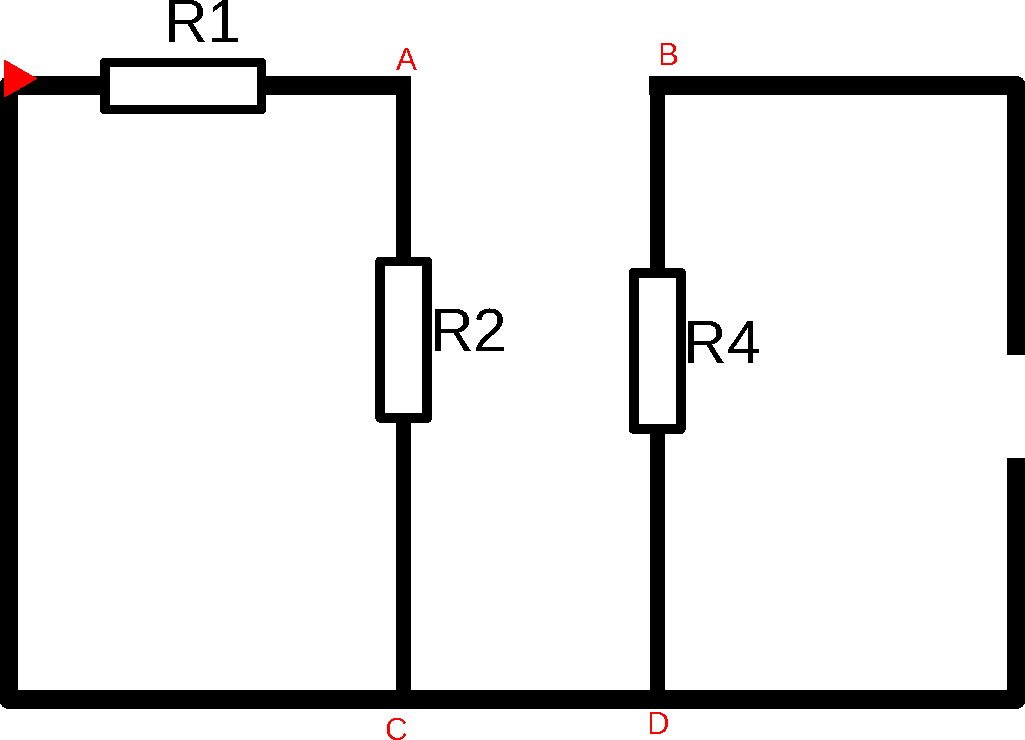
\includegraphics[scale=0.3]{methode-2-4}

La résistance équivalente  vaut donc \(R_1//R_2 + R_4 = \frac{R_1R_2}{R_1+R_2} + R_4\)

La tension \(E_{th} = U_{AB}\), vaut elle, \(U_{AC} = U_{R_2} + I_sR_4\). En appliquant un pont diviseur de tension, on trouve \(U_{R_2} = E_1\times \frac{R_2}{R_2+R_1}\).

Une fois le circuit modélisé par son équivalent de Thévenin avec les valeurs trouvées, on n'a plus qu'à appliquer un pont diviseur de tension pour trouver tension à la résistance, puis le courant : \(U_3 = E_{th}\frac{R_3}{R_3+R_{th}}\), donc \(I = \frac{U_3}{R_3}\).

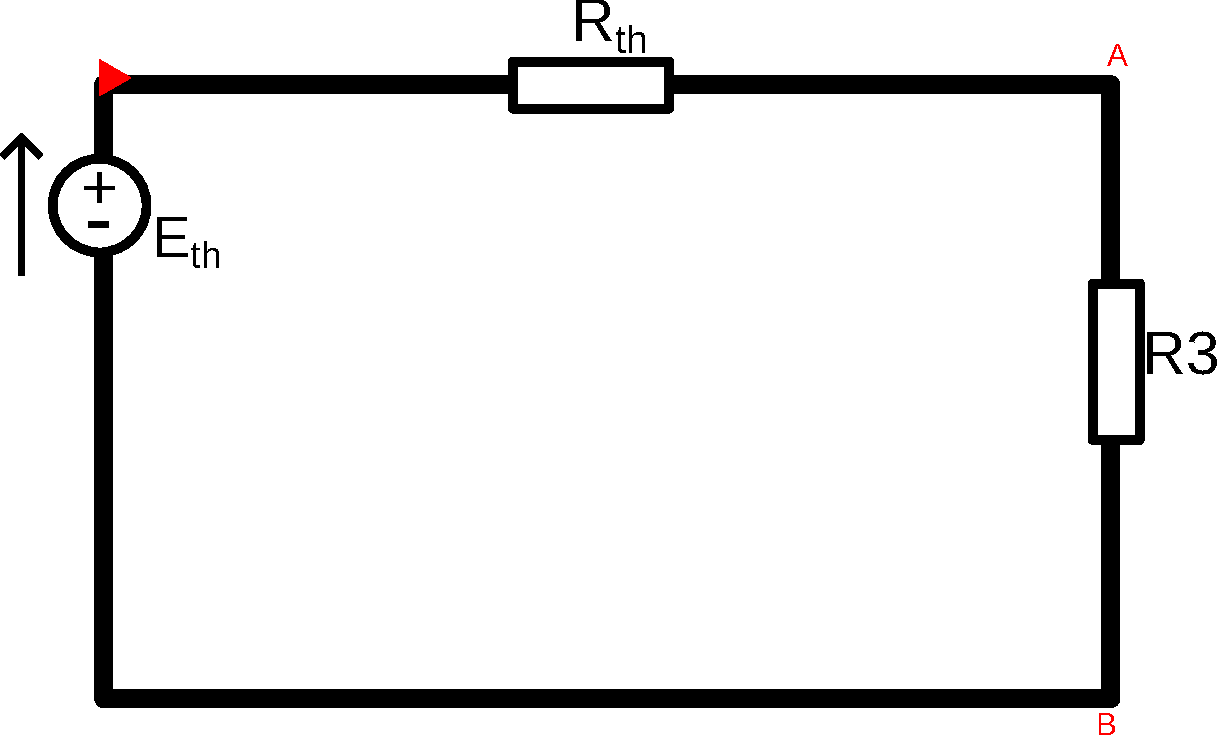
\includegraphics[scale=0.3]{methode-2-5}
\section{Appliquer le théorème de Milmann}
Dans cet exempple, pour trouver la tension MN, on peut, en plus des méthodes utilisées plus haut, utiliser le théorème de Milmann.

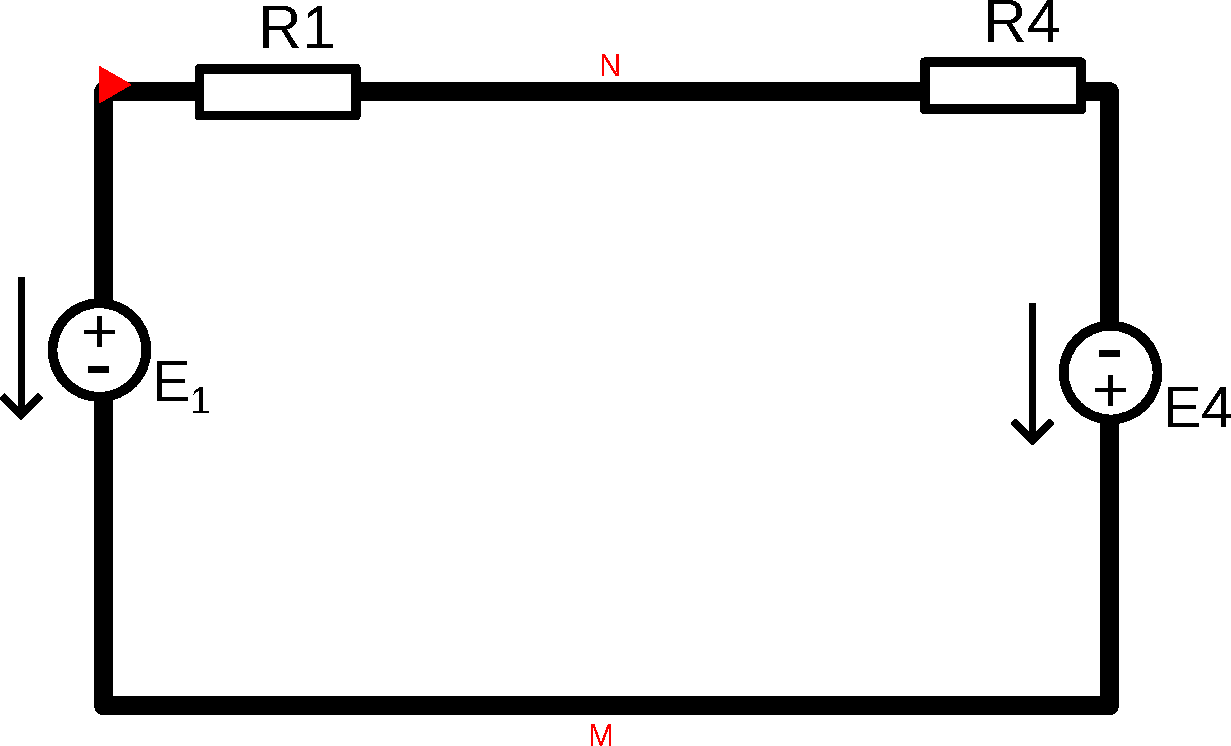
\includegraphics[scale=0.3]{methode-2-7}

En supposant que le potentiel est nul au point M, on peut donc écrire \(U_{NM} = \frac{\frac{E_1}{R_1}+ \frac{E_4}{R_4}}{\frac{1}{R_1}+\frac{1}{R_4}}\).
\end{document}

